%%%%%%%%%%%%%%%%%%%%%%% file template.tex %%%%%%%%%%%%%%%%%%%%%%%%%
%
% This is a general template file for the LaTeX package SVJour3
% for Springer journals.          Springer Heidelberg 2010/09/16
%
% Copy it to a new file with a new name and use it as the basis
% for your article. Delete % signs as needed.
%
% This template includes a few options for different layouts and
% content for various journals. Please consult a previous issue of
% your journal as needed.
%
%%%%%%%%%%%%%%%%%%%%%%%%%%%%%%%%%%%%%%%%%%%%%%%%%%%%%%%%%%%%%%%%%%%
%
% First comes an example EPS file -- just ignore it and
% proceed on the \documentclass line
% your LaTeX will extract the file if required
\begin{filecontents*}{example.eps}
%!PS-Adobe-3.0 EPSF-3.0
%%BoundingBox: 19 19 221 221
%%CreationDate: Mon Sep 29 1997
%%Creator: programmed by hand (JK)
%%EndComments
gsave
newpath
  20 20 moveto
  20 220 lineto
  220 220 lineto
  220 20 lineto
closepath
2 setlinewidth
gsave
  .4 setgray fill
grestore
stroke
grestore
\end{filecontents*}
%
\RequirePackage{fix-cm}
%
%\documentclass{svjour3}                     % onecolumn (standard format)
\documentclass[smallcondensed]{svjour3}    % onecolumn (ditto)
%\documentclass[smallextended]{svjour3}       % onecolumn (second format)
%\documentclass[twocolumn]{svjour3}          % twocolumn

%
\smartqed  % flush right qed marks, e.g. at end of proof
%
\usepackage{graphicx}
%
% \usepackage{mathptmx}      % use Times fonts if available on your TeX system
%
% insert here the call for the packages your document requires
%\usepackage{latexsym}
\usepackage{dcolumn}% Align table columns on decimal point
\usepackage{bm}% bold math
\setlength{\marginparwidth}{2cm}
\usepackage{changes}
\usepackage{bbm}
%\usepackage[mathlines]{lineno}% Enable numbering of text and display math
%\linenumbers\relax % Commence numbering lines
\usepackage[utf8]{inputenc}
\usepackage[T1]{fontenc}
\usepackage{mathptmx}
\usepackage{amsmath}
\usepackage{amssymb}
\usepackage{statmath}
\usepackage[numbers]{natbib}
\usepackage{hyperref}
\usepackage{enumitem}
\usepackage{mathtools}
\usepackage{siunitx}
\DeclarePairedDelimiter\ceil{\lceil}{\rceil}
%
% please place your own definitions here and don't use \def but
\newcommand{\mytilde}{\raise.17ex\hbox{$\scriptstyle\mathtt{\sim}$}}
%
% Insert the name of "your journal" with
\journalname{Nonlinear Dynamics}
%
\begin{document}

\title{Recurrence spike spectra}

\titlerunning{Recurrence spike spectra}        % if too long for running head

\author{K. Hauke Kraemer \and
		Frank Hellmann \and
		Mehrnaz Anvari \and
        J\"urgen Kurths \and 
        Norbert Marwan
}


\institute{K. Hauke Kraemer \and J\"urgen Kurths \and Norbert Marwan \and Frank Hellmann \at Potsdam Institute for Climate Impact Research, Member of the Leibniz Association, 14473 Potsdam, 
Germany \email{hkraemer@pik-potsdam.de}\and
           K. Hauke Kraemer \and J\"urgen Kurths \at Institute of Physics and Astronomy, University of Potsdam, 14476 Potsdam, Germany \and
		   Norbert Marwan \at Institute of Geosciences, University of Potsdam, 14476 Potsdam, Germany \and
		   J\"urgen Kurths \at Institute of Physics, Humboldt Universit\"at zu Berlin, 12489 Berlin, Germany
}

\date{Received: date / Accepted: date}
% The correct dates will be entered by the editor


\maketitle

\begin{abstract}
A novel kind of power spectrum is constructed, the \textit{inter spike spectrum}, which transforms any signal into its spike-frequency domain. This method 
clearly shows the apparent cycles in the data and overcomes the problems for spike-train-like signals when using the obvious idea of Fourier-transforming it. 
We invent this instructive approach with the 
idea of transforming the $\tau$-recurrence rate of a recurrence plot (RP), which often has a spiky appearance. The $\tau$-recurrence rate is the density of recurrence points 
along diagonals of the RP, which are parallel to the main diagonal with a distance of $\tau$. In this context the inter spike spectrum can be interpreted as a nonlinear power 
spectrum of a potentially high dimensional system which constitutes the RP. The proposed measure is robust to noise and is able to detect and analyze bifurcations.

\keywords{Bifurcations \and Recurrence Analysis \and Decomposition \and Frequency Analysis}
\PACS{05.45.Tp, 05.90.+m, 89.90.+n, 02.70.Uu, 05.10.Ln, 05.45.-a, 05.45.Ac}
\end{abstract}

\section{Introduction}\label{sec_tau_rr_intro}

Recurrence Plots (RPs) provide a vivid representation of complex dynamics stemming from potentially high dimensional systems, Eq.~\eqref{eq_rp_definition}. 
\begin{equation}\label{eq_rp_definition}
R_{i,j}(\varepsilon) = \Theta\left(\varepsilon - D_{i,j}\right) 
= \Theta\left(\varepsilon - \| \vec{x}_i - \vec{x}_j\|\right), \qquad \vec{x} \in \mathbb{R}^d, \quad i,j \in [1,\ldots, N].
\end{equation}
The simple idea to 
track recurring states of the $d$-dimensional trajectory $\vec{x}_i$ of the system under study not only allows for a beneficial visualization of the dynamics, but also for its 
quantification, using certain structures in the RP, such as diagonal or vertical lines \cite{marwan2007}. 

Some of these recurrence quantification measures, the entropy of diagonal lines and the entropy of 
recurrence times, can be related to the Kolmogorov-Sinai entropy \cite{march2005,baptista2010}. However, these quantifiers have a free parameter, the minimal considered line length, and 
are usually biased, due to the finite size of the RP and thickened diagonal lines, which needs to be corrected \cite{Kraemer2019}. Moreover, the mentioned statistics cannot account for 
changing regular (non-chaotic) dynamics, such as period-doubling bifurcations.
A rather simple idea is to look at the $\tau$-recurrence rate of the RP ($\tau$-RR, Eq.~\ref{eq_tau_rr}) \cite{marwan2002pla,Zbilut2008}.
This is the density of recurrence points along the diagonals of the recurrence matrix, as a function of the distance $\tau$ (sampling units) to the main diagonal:
\begin{equation}\label{eq_tau_rr}
\tau\text{-RR}(\varepsilon) = RR(\tau, \varepsilon) = \frac{1}{N-\tau} \sum_{i=1}^{N-\tau	} R_{i,i+\tau}.
\end{equation}
$\tau$-RR serves as an estimator for the probability that the system recurs after time $\tau \Delta t$, with $\Delta t$ being the sampling time of the trajectory 
$\vec{x}_i = \vec{x}(\Delta t \cdot i),\, i=1,\ldots,N$. 
\citet{Zbilut2008} pointed out that $\tau$-RR could be used as a plugin value for the auto-correlation function $C(\tau)$ and, hence, via the Wiener-Khinchim theorem a 
``generalized'' powerspectrum can be obtained. This is reasonable, since the average distances for a given lag $\tau$ 
\begin{equation}
\overline{D}(\tau) = \frac{1}{N-\tau}\sum_{i=1}^{N-\tau} D_{i, i+\tau}
\end{equation}
can be directly read from the distance matrix $\mathbf{D}$ and is also preserved in its thresholded version $\tau$-RR. There are clear advantages for a recurrence-derived 
powerspectrum, i.e., Fourier transforming (FT) $\tau$-RR (Fig.~\ref{fig_tau_rr_spectrum_example}D), instead 
of $C(\tau)$ (Fig.~\ref{fig_tau_rr_spectrum_example}C): There are no assumptions for stationarity or sampling, when constructing a RP.
Furthermore, the correlation structures of higher dimensional spaces can be resolved in the recurrence-derived Fourier-spectrum.\\

\begin{figure}
 \centering
 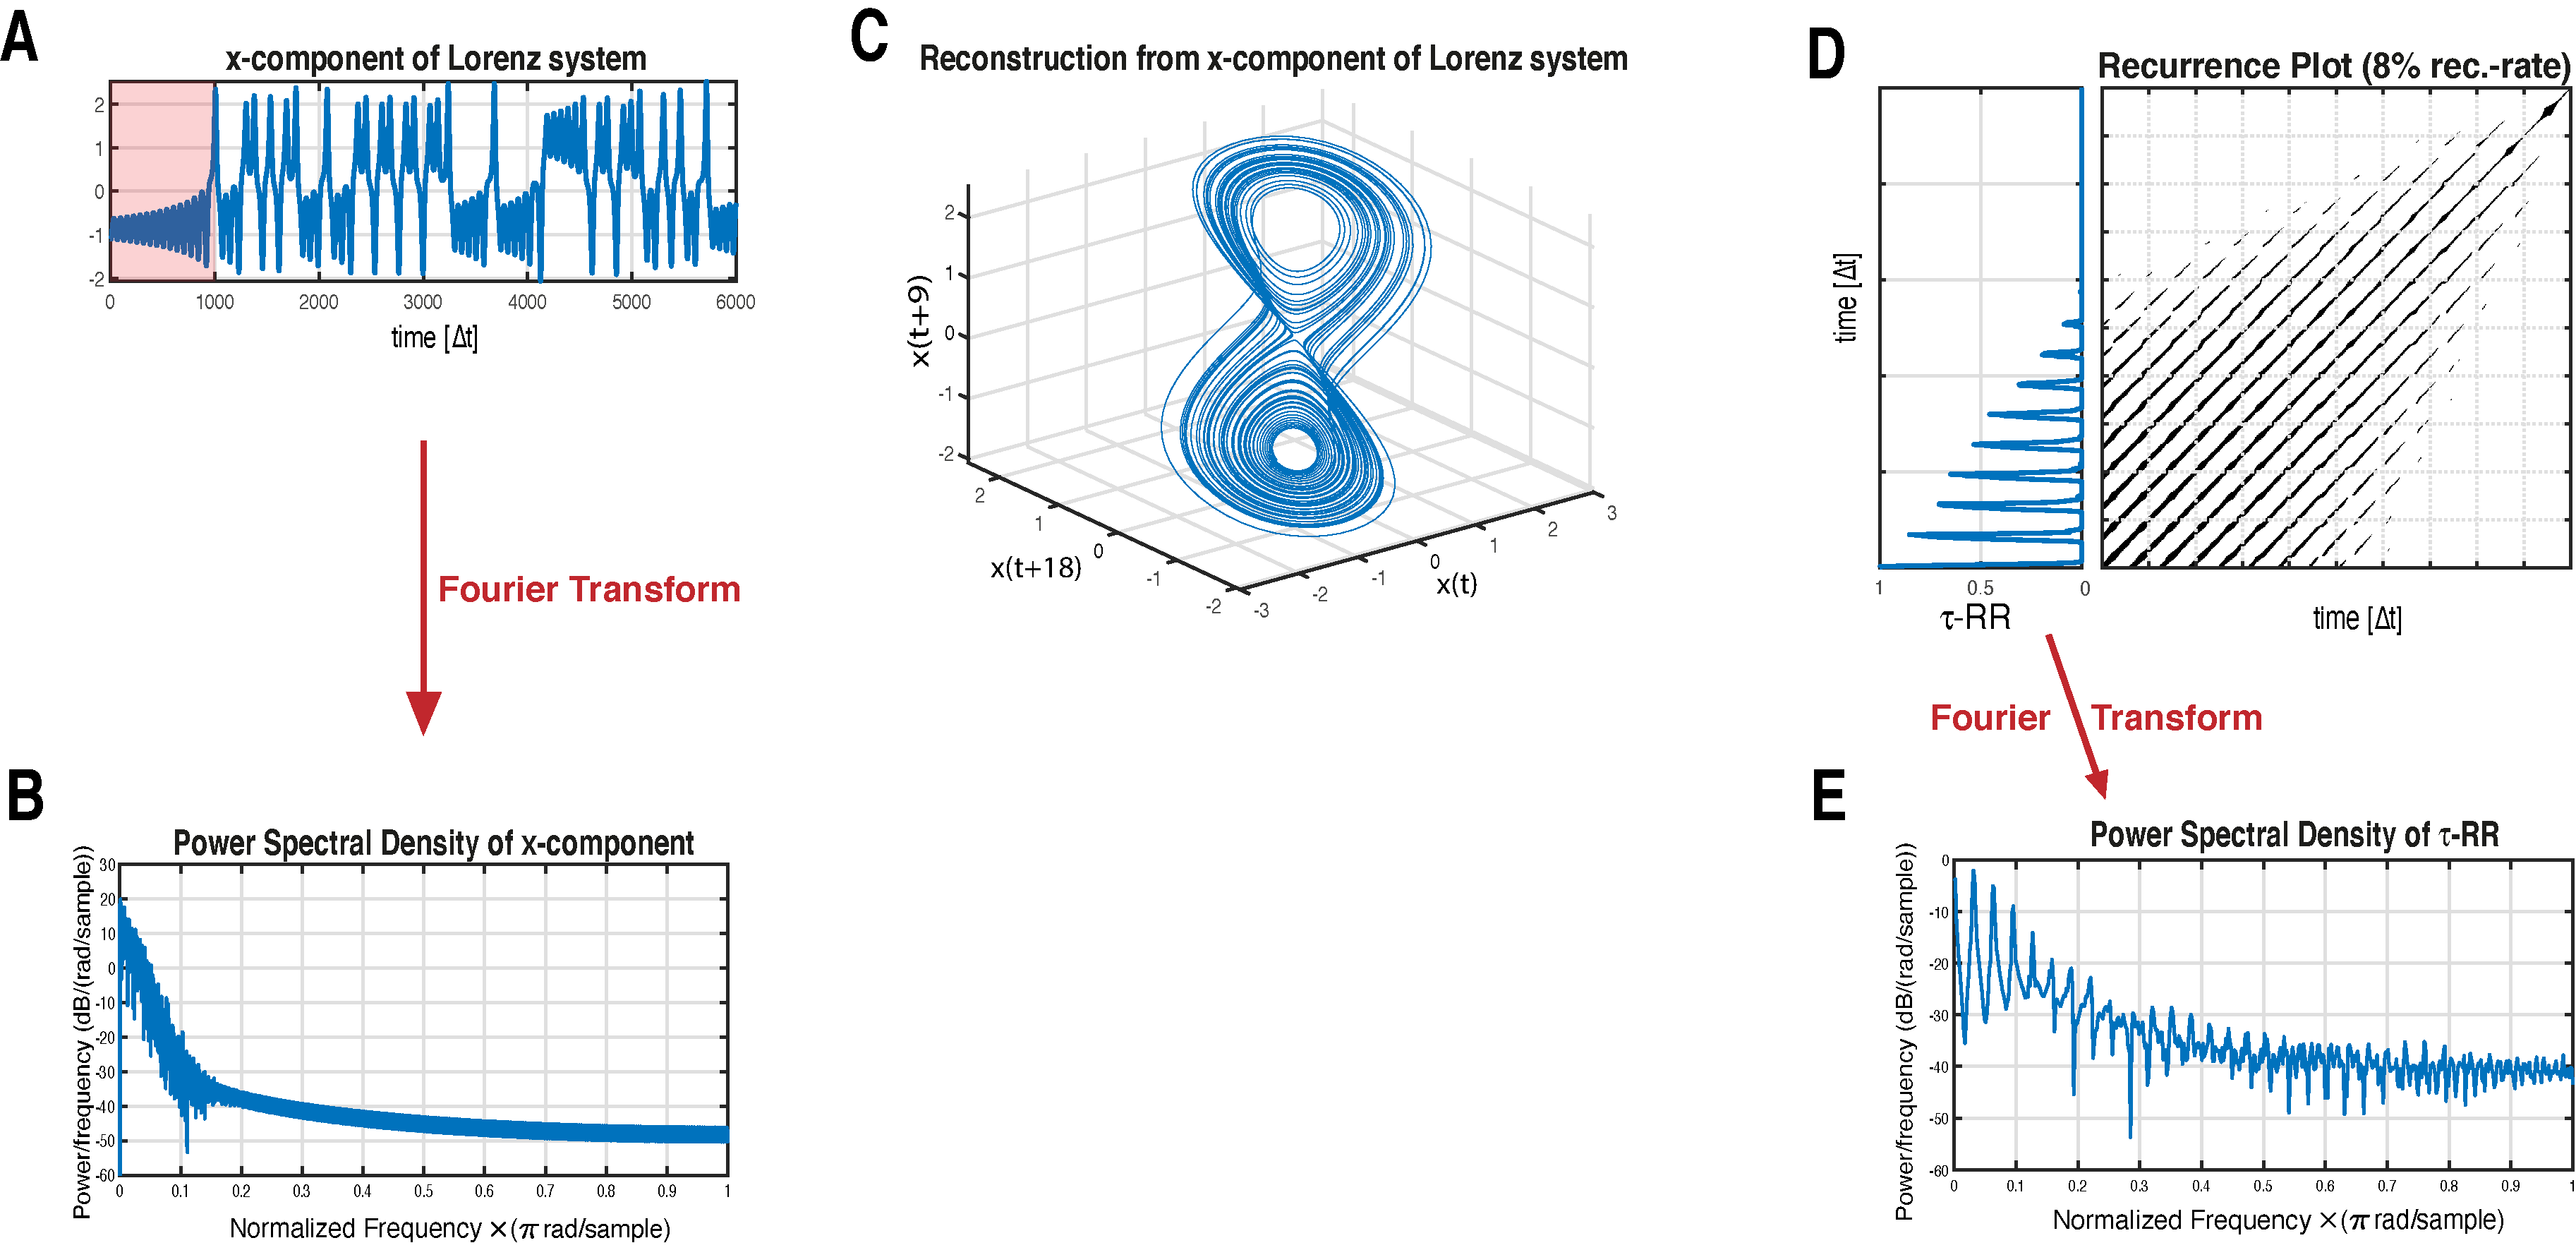
\includegraphics[width=0.9\textwidth]{./figures/fig_tau_rr_spectrum_example}
 \caption{Schematic illustration of a $\tau$-recurrence rate based spectrum. \textbf{A} $x$-component time series of the Lorenz63-System (Eq.~\eqref{eq_model_Lorenz63}) and 
 \textbf{B} its corresponding Fourier power spectrum. 
 \textbf{C} Reconstructed state space portrait from the time series shown in \textbf{A} using PECUZAL time-delay embedding \cite{Kraemer2021}. 
 \textbf{D} Subset of the recurrence plot and the corresponding $\tau$-recurrence rate obtained from the state space trajectory in \textbf{C}. The shaded interval in the time series in \textbf{A} corresponds to the shown subset. 
 \textbf{E} Fourier Power spectrum obtained from the $\tau$-recurrence (subset shown in panel \textbf{D}) \cite{Zbilut2008}.
 }\label{fig_tau_rr_spectrum_example}
\end{figure}

However, there is a drawback to this approach. Whenever $\tau$-RR is a spike-train-like signal, which it is in most cases (see Fig.~\ref{fig_tau_rr_spectrum_example}) especially for 
map-data (low-resolution data), a FT of such a signal leads to a spike-train-like image in the frequency domain (e.g. \cite{Schild1982,Cordoba1989}, see 
Fig.~\ref{fig_tau_rr_spectrum_example}D). Thus, it is not intuitive how to extract meaningful information about dominant frequencies of the systems' state space trajectory. 

For clarification, consider the signal we would like to analyze 
(e.g. the $\tau$-RR of a system) to be a Dirac comb (DC) with inter-spike period $T_\text{is}$: 
\begin{equation}
\text{DC}_{\text{is}}(t) = \sum_{k=-\infty}^{\infty} \delta(t-kT_\text{is}),
\label{eq_dirac_comb}
\end{equation}
i.e., a series of Dirac delta functions for a period $T_\text{is}$. There is only one single period -- $T_\text{is}$ -- in this signal (Fig.~\ref{fig_tau_rr_dirac_comb}A, D), so 
in principle we would strive for a single peak in the frequency domain of this signal at a frequency $f=1/T_\text{is}$. Surprisingly the Fourier spectrum does not meet this expectation 
and instead of a single frequency, there are exceptionally many frequencies excited (Fig.~\ref{fig_tau_rr_dirac_comb}B, E). This is, because the Fourier components add constructively 
for every frequency $1/T_\text{is}$ and therefore $\text{DC}_{\text{is}}(t)$ coincides with its own Fourier transform up to a factor $1/T_\text{is}$.

\begin{figure}[h]
 \centering
 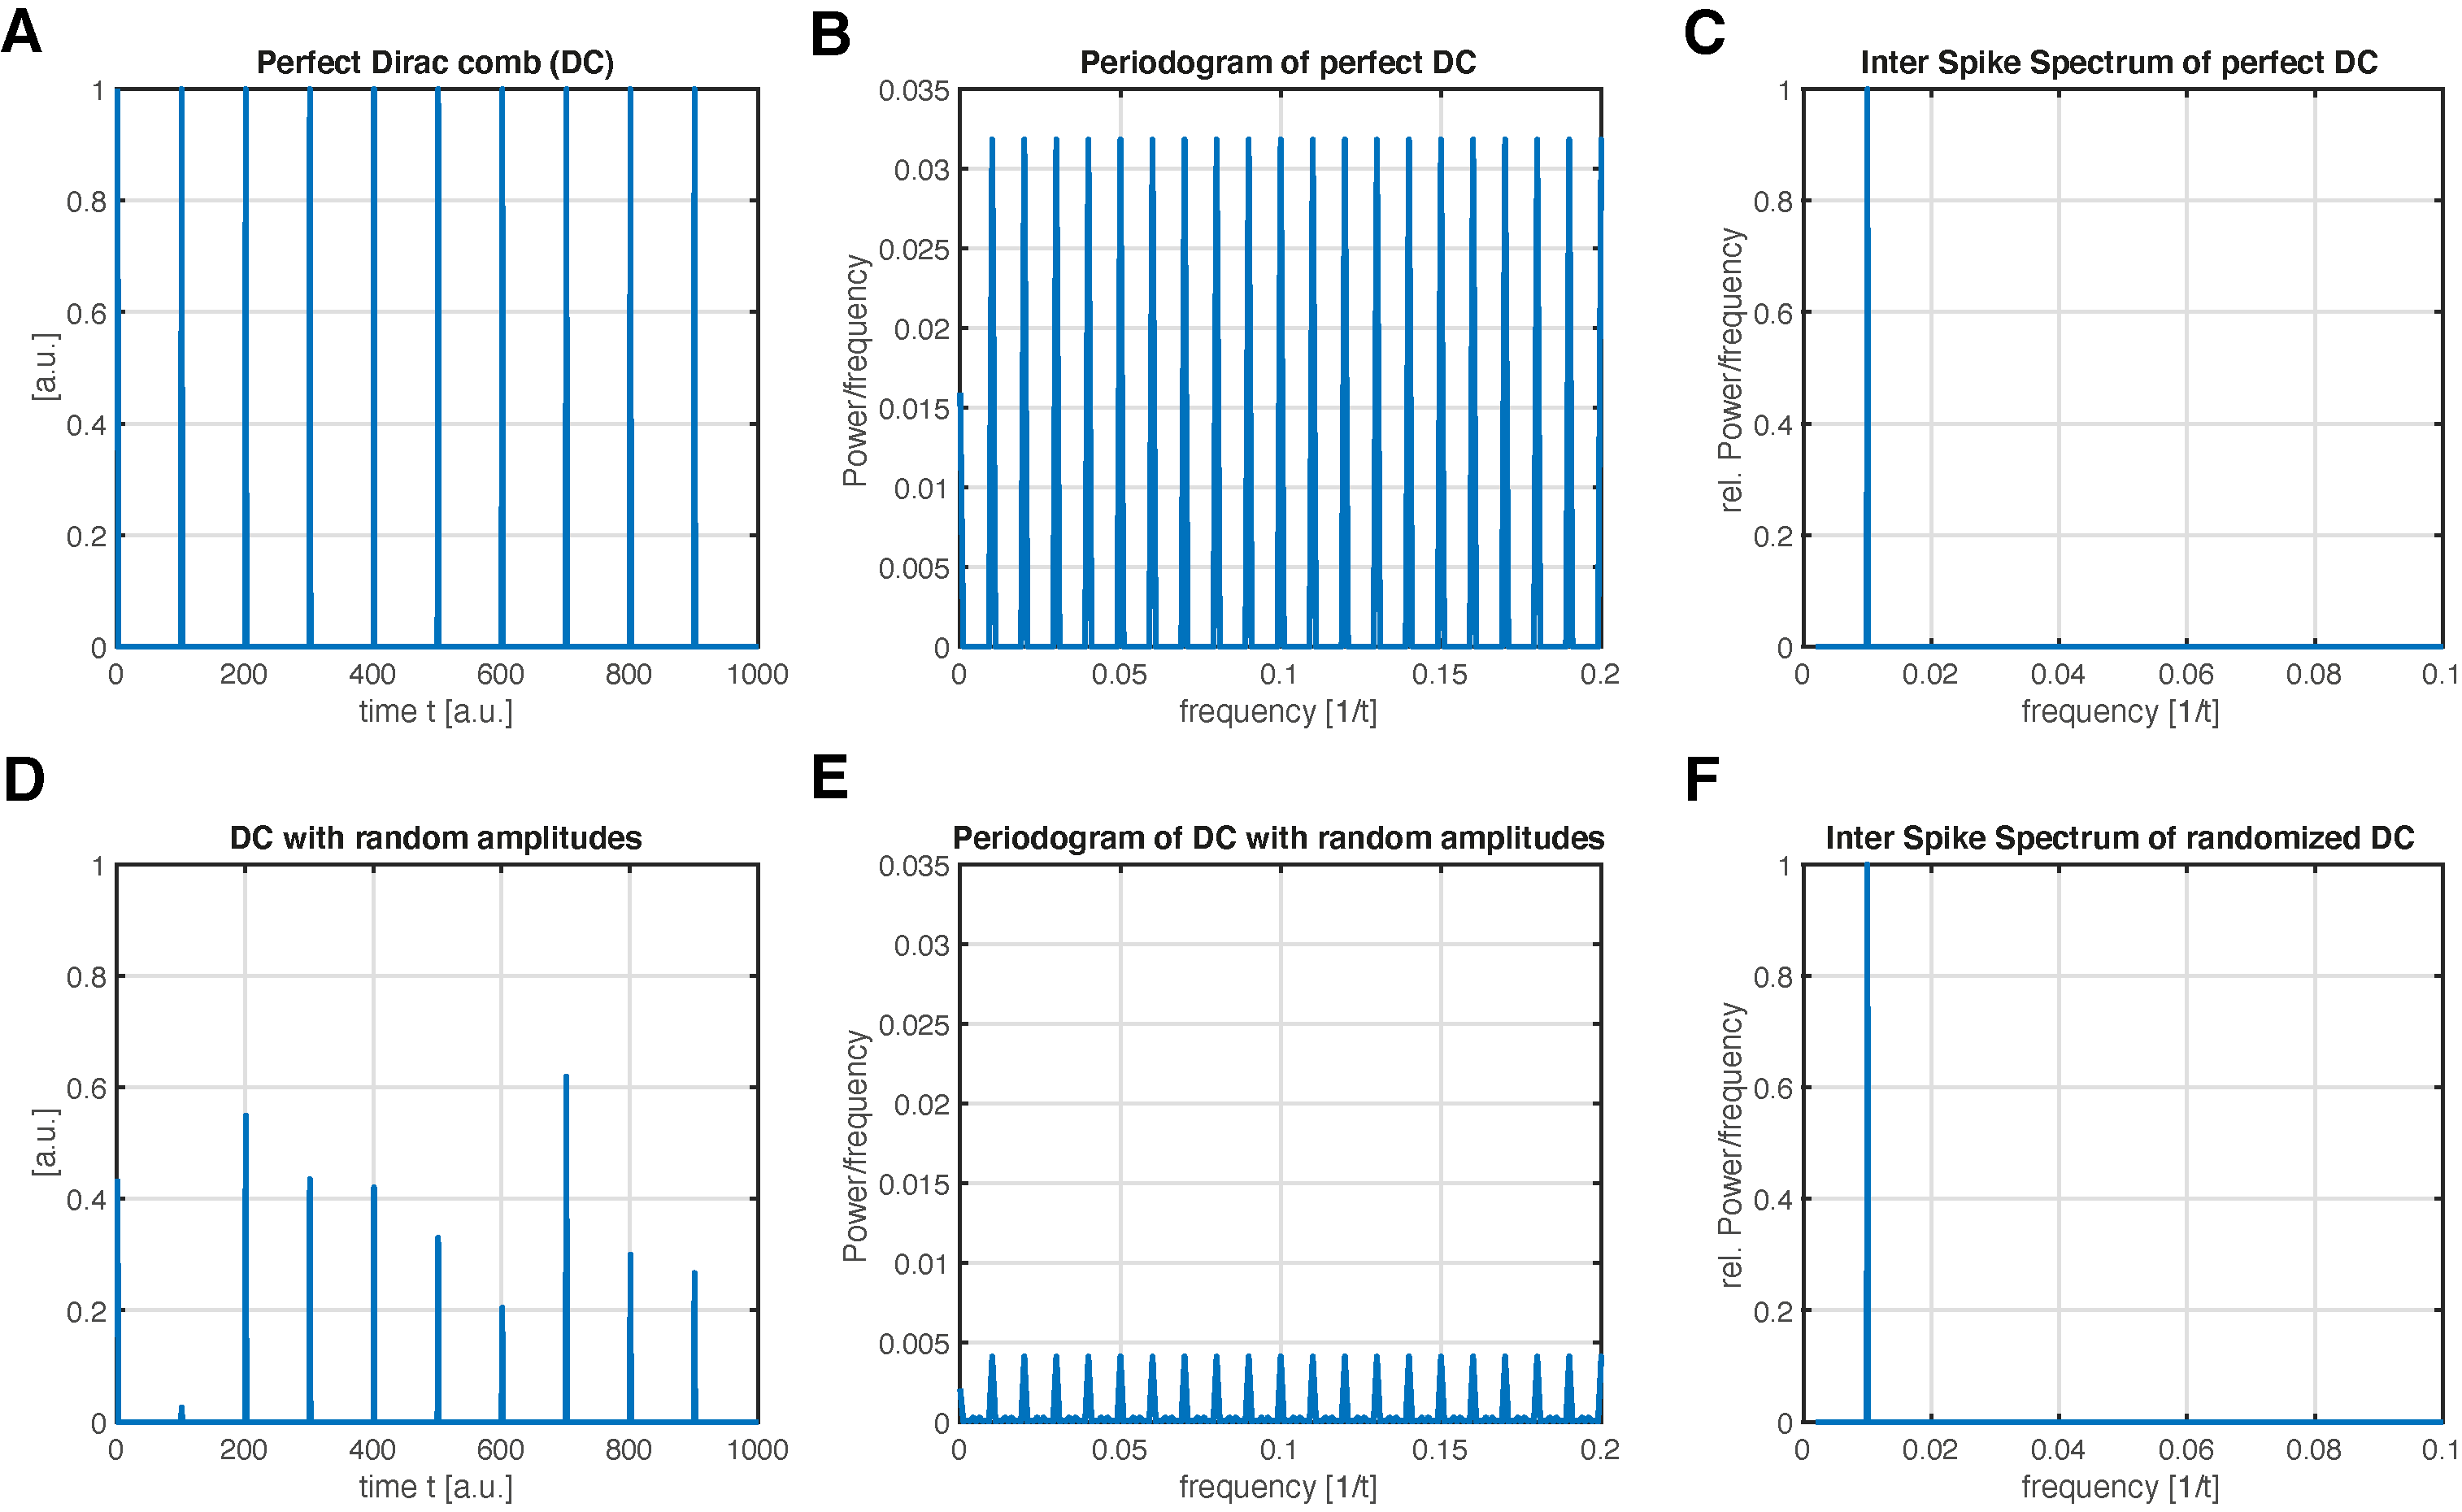
\includegraphics[width=0.9\textwidth]{./figures/fig_tau_rr_dirac_comb}
 \caption{The transformation of a Dirac comb (series of Dirac delta functions) with a single inter-spike period $T_{\text{is}}=100$ ($\widehat{=}f=0.01$) 
 into the frequency domain. 
 \textbf{A} Dirac Comb (DC) with equal amplitudes and
 \textbf{B} its FFT-based powerspectrum.
 \textbf{C} Proposed inter spike spectrum of the signal in \textbf{A} showing a single frequency, which corresponds to the inter-spike period $T_{\text{is}}$ ($f=0.01$).
 \textbf{D} DC with randomly chosen amplitudes and same $T_{\text{is}}$ as in \textbf{A}, and
 \textbf{E} its FFT-based powerspectrum. 
 \textbf{F} Proposed inter spike spectrum of the signal in \textbf{D} showing a single frequency, which corresponds to the expected inter-spike period $T_{\text{is}}$ ($f=0.01$). 
 Inter spike spectra were obtained with a LASSO regression and a regularization threshold corresponding to $\rho=0.9$ accordance of the signals in (\textbf{A},\textbf{D}) and 
 its re-composed signals (c.f. Section~\ref{sec_tau_rr_method}). 
}
\label{fig_tau_rr_dirac_comb}
\end{figure}

In this article we propose a new way of transforming a spike-train-like signal into its frequency domain. This novel \textit{inter spike spectrum} does not show resonance 
behavior of the signal's inherent inter-spike frequencies (Fig.~\ref{fig_tau_rr_dirac_comb}C, F). Section \ref{sec_tau_rr_method} explains the idea, which can be used to decompose 
any arbitrary signal and is not restricted to the $\tau$-RR, which we exemplify here. However, the more spiky the signal is, the more outstanding our new approach is compared to a 
FT. In Section \ref{sec_tau_rr_application} we exemplify its use when transforming the $\tau$-RR of a system under study. In this case, the inter spike spectrum can unravel 
characteristic time scales of high dimensional systems, which is not possible when using a FT.

\section{Method}\label{sec_tau_rr_method}
    
The signal, which we would like to transform -- we focus on $\tau$-RR in this article, but this can be applied to any sort of signal -- 
is decomposed into a set of appropriate basis functions. Instead of using trigonometric functions, as it is the idea in the Fourier decomposition, we use Dirac combs (DC) with 
different inter-spike periods as basis functions, Eq.~\eqref{eq_dirac_comb}. Let $s(t_i)$ be the normalized signal we want to transform with length $N$ and 
$t_i=i\cdot \Delta t,~i=1,\ldots,N$, where $\Delta t$ denotes the sampling time and $s(t_i) \in [0,\ 1]\ \forall\ i$. In the following we label this time series as a $(1\times N)$-dimensional 
vector $\bf{s}$. 
First, $\tilde{N}$ different DC's of length $N$ are constructed with inter-spike periods $T_\text{is} \in [1,\ldots,\tilde{N}]$ and $\tilde{N}=\ceil*{N/2}+1$. Second, in order to account 
for possible phase shifts of 
these basis functions occurring in $\bf{s}$, each of these $\tilde{N}$ different DC's also need to be shifted one step further $T_\text{is}-1$ times. This leaves us with a total number of 
$M = \sum_{i=1}^{\tilde{N}}i$ 
basis functions which we can arrange as rows of a $(M\times N)$-sized matrix $\bfX$
(Fig.~\ref{fig_tau_rr_basis_functions}A illustrates the described procedure)
\begin{align}
\bfX_{i,j} &= \sum_{k=0}^{N}\delta\left(j-1-kT(i)-i+T(i) \right), \quad i=1,\dots,\ceil*{N/2}+1, \quad j=1,\dots,N\\
T(i)&= n \quad, \forall n:~ \frac{n(n-1)}{2} + 1 \leq i <  \frac{n(n+1)}{2} + 1,\quad n \in \mathbb{N}_+.
\label{eq_basis_matrix}
\end{align}
Note that due to the shifting of each of the basis functions of inter-spike period $T_\text{is}$, $\bfX$ is not linear independent anymore. 
Furthermore, there will be identical basis functions and also basis functions, which do not allow for a unambiguous inter spike period, 
if we would include all $N$ possible inter spike periods for a signal of length $N$ instead of $\ceil*{N/2}+1$ (Fig.~\ref{fig_tau_rr_basis_functions}A). 
The reason is that in contrast to a trigonometric decomposition, where the Nyquist frequency marks a lower bound for the corresponding wave period, here 
the maximum considered inter spike period is bounded by $T_{\text{is}}^{\text{max}} = \ceil*{N/2}+1$ (schematically illustrated in 
Fig.~\ref{fig_tau_rr_basis_functions}B).\\ 

\noindent Eventually, an under-determined linear system
\begin{equation}
\bf{X}^T\bf{\beta}=\bf{s}
\label{eq_linear_system}
\end{equation}  
has to be solved for $\bf{\beta}$, a $(M\times 1)$-sized vector carrying the loadings we are interested in. Along a variety of algorithms which can solve this problem, we are 
particularly interested in those solutions, which promote sparsity in $\bf{\beta}$, since our goal is to decompose the signal $\bfs$ into a minimal number of basis 
functions (for an excellent overview of the topic we refer to \citet{Brunton2019}). In this paper we either use the \textit{least absolute shrinkage and selection operator} 
(LASSO) \cite{Tibshirani1996} or a \textit{sequentially thresholded least squares} (STLS) regression \cite{Brunton2016,Brunton2019} to obtain a solution $\hat{\bf{\beta}}$. Finally, we group loadings 
which correspond to basis functions having the same period 
$T_\text{is}$ into $\hat{\bf{\beta}}_f$ and obtain the 
\textit{inter spike spectrum} by simply plotting $\hat{\bf{\beta}}_f$ as a function of the frequency $f=T_\text{is}^{-1}$, with $T_\text{is}=\Delta t, 2\Delta t, \dots, (\ceil*{N/2}+1) \Delta t$ 
(Fig.~\ref{fig_tau_rr_dirac_comb}C, F).

\begin{figure}
\centering
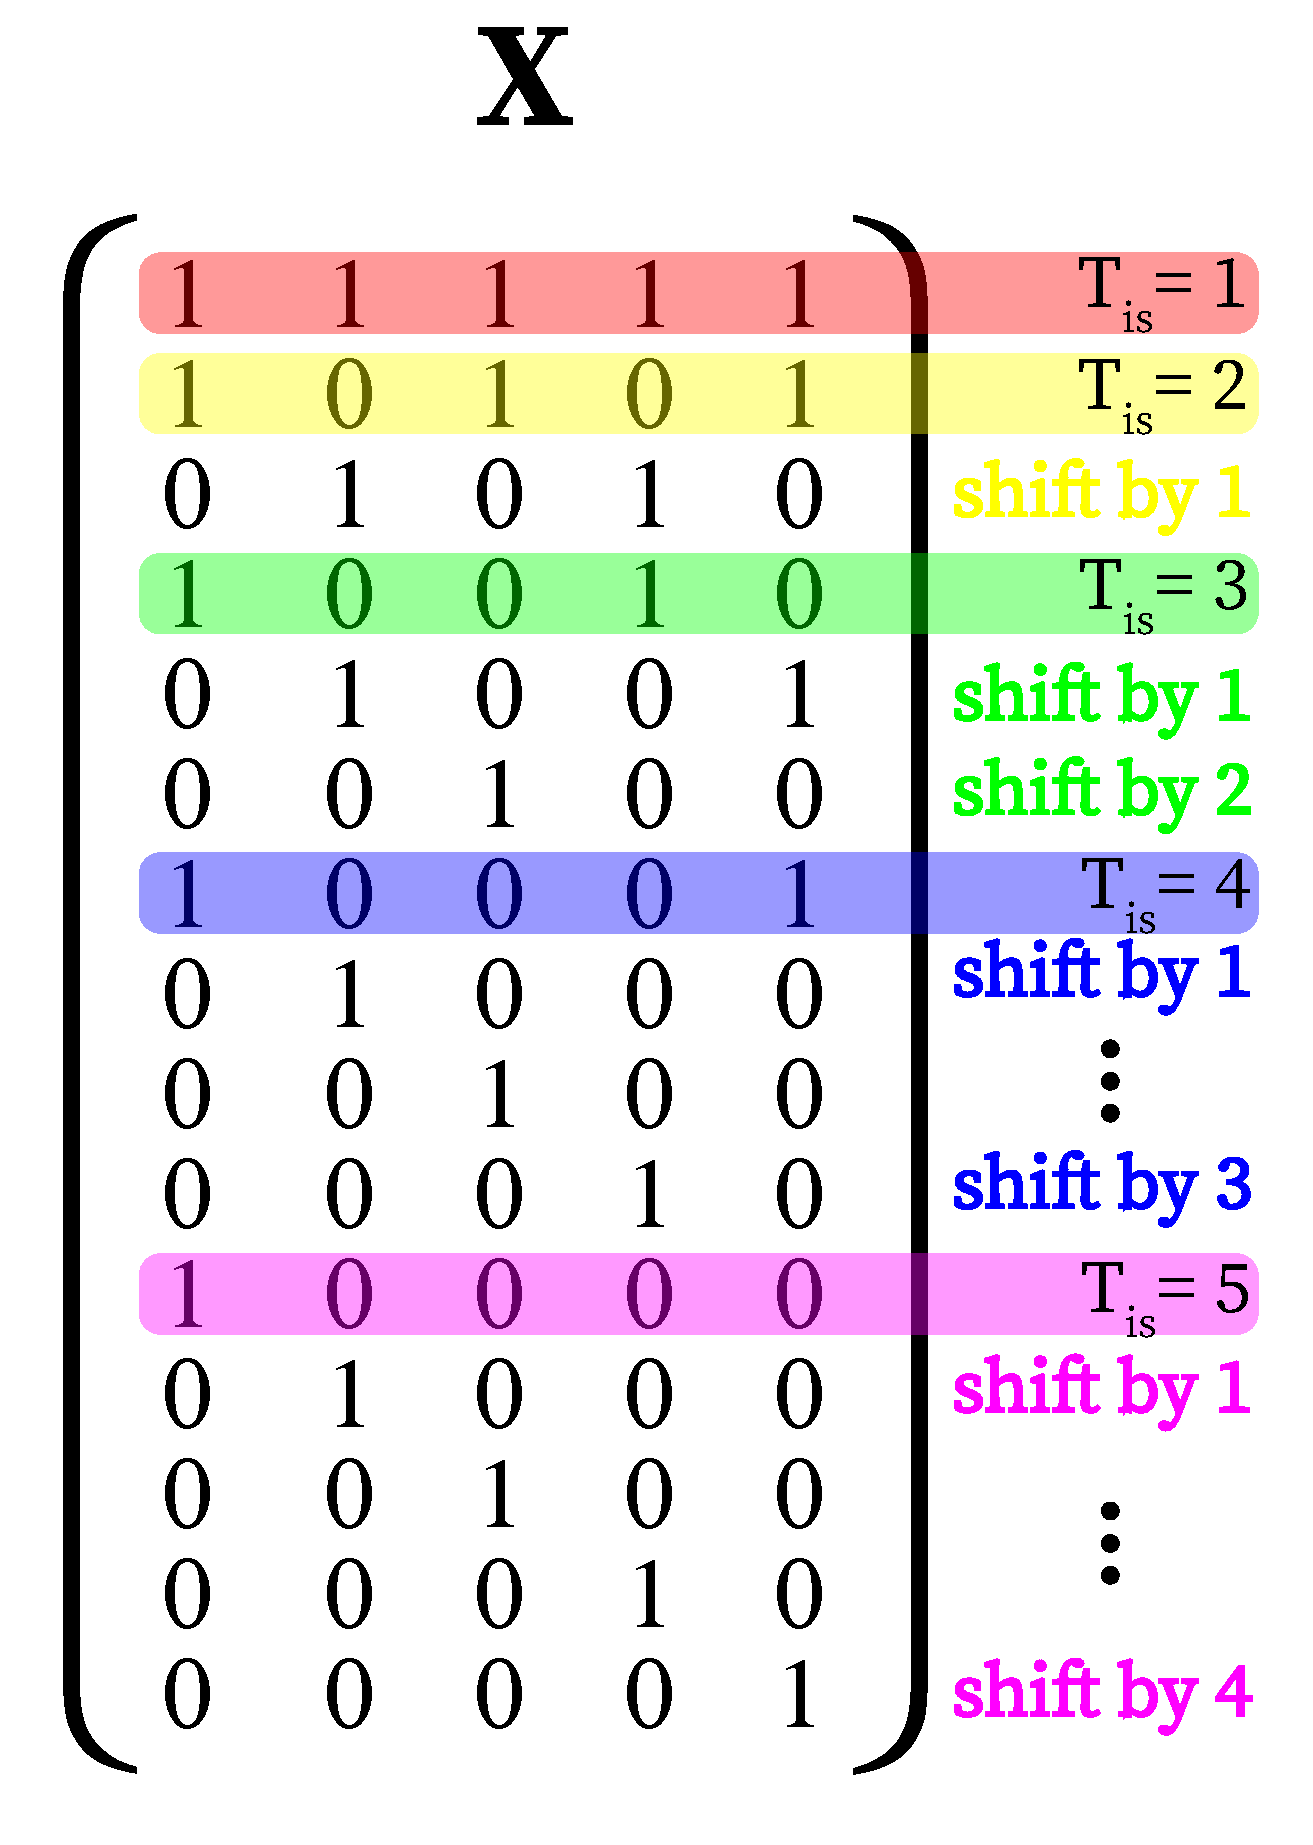
\includegraphics[width=0.9\textwidth]{./figures/fig_tau_rr_basis_functions}
\caption{\textbf{A} Example for a full set of basis functions for an input signal of length $N=4$, aligned in the matrix $\bfX'$. Inter spike periods $T_{\text{is}}$ larger 
than $\ceil*{N/2}+1$ lead to redundant basis functions (i.e., repeated lines in $\bfX$, red sheared) or basis functions, which can not be uniquely assigned to a certain inter spike period 
(blue sheared). \textbf{B} The final set of unambiguous, but still linearly dependent, basis functions aligned in the matrix $\bfX$.} \label{fig_tau_rr_basis_functions}
\end{figure}

In addition to the computational complexity of solving Eq.~\eqref{eq_linear_system}, the proposed method must also deal with the free choice of the regression regularization parameter $\alpha$, 
which determines the sparsity of the regression coefficient vector $\hat{\bf{\beta}}$. Obviously, there will be numerous peaks in the inter spike spectrum of a given signal, when $\alpha$ is small, 
since $\alpha=0$ corresponds to the least squares solution and the corresponding $\hat{\bf{\beta}}$ is an exact solution of Eq.~\ref{eq_linear_system} and not sparse. On the other hand, only a sparse number 
of non-zero loadings in $\hat{\bf{\beta}}$ -- \textit{aka} peaks in the inter spike spectrum -- are obtained when $\alpha$ is sufficiently large. In this paper we select $\alpha$ such that the 
re-composed signal $\tilde{\bf{s}}=\bf{X}^T\hat{\bf{\beta}}$ matches a given (Pearson) correlation coefficient $\rho$ between the original signal $\bf{s}$ and itself.

\section{Application}\label{sec_tau_rr_application}

We exemplify the use of the inter spike spectrum in combination with the $\tau$-RR as outlined in 
Section \ref{sec_tau_rr_intro} on several interesting research questions. The procedure is the following:
\begin{itemize}[noitemsep]
\item[(1)] Compute a RP of the trajectory of the system, Eq.~\eqref{eq_rp_definition}. 
\item[(2)] Compute the $\tau$-RR of that RP, Eq.~\eqref{eq_tau_rr}.
\item[(3)] Transform the $\tau$-RR into the proposed inter spike spectrum, see Section \ref{sec_tau_rr_method}.
\end{itemize}

\subsection{Period estimation for different dynamics in the R\"ossler system}
First, we consider the R\"ossler system (Eq.~\eqref{eq_model_roessler} in Appendix \ref{sec_models_roessler}) 
in three different dynamical setups. We use the proposed inter spike spectrum to
identify the type of dynamics.
We set the parameters $b=2$, $c=4$ and analyze period-2 limit cycle dynamics ($a=0.36$, Fig.~\ref{fig_tau_rr_example_roessler}A, D, G, J), 
period-3 limit cycle dynamics ($a=0.41$, Fig.~\ref{fig_tau_rr_example_roessler}B, E, H, K) and chaotic dynamics ($a=0.428$, Fig.~\ref{fig_tau_rr_example_roessler}C, F, I, L).  

\begin{figure}
 \centering
 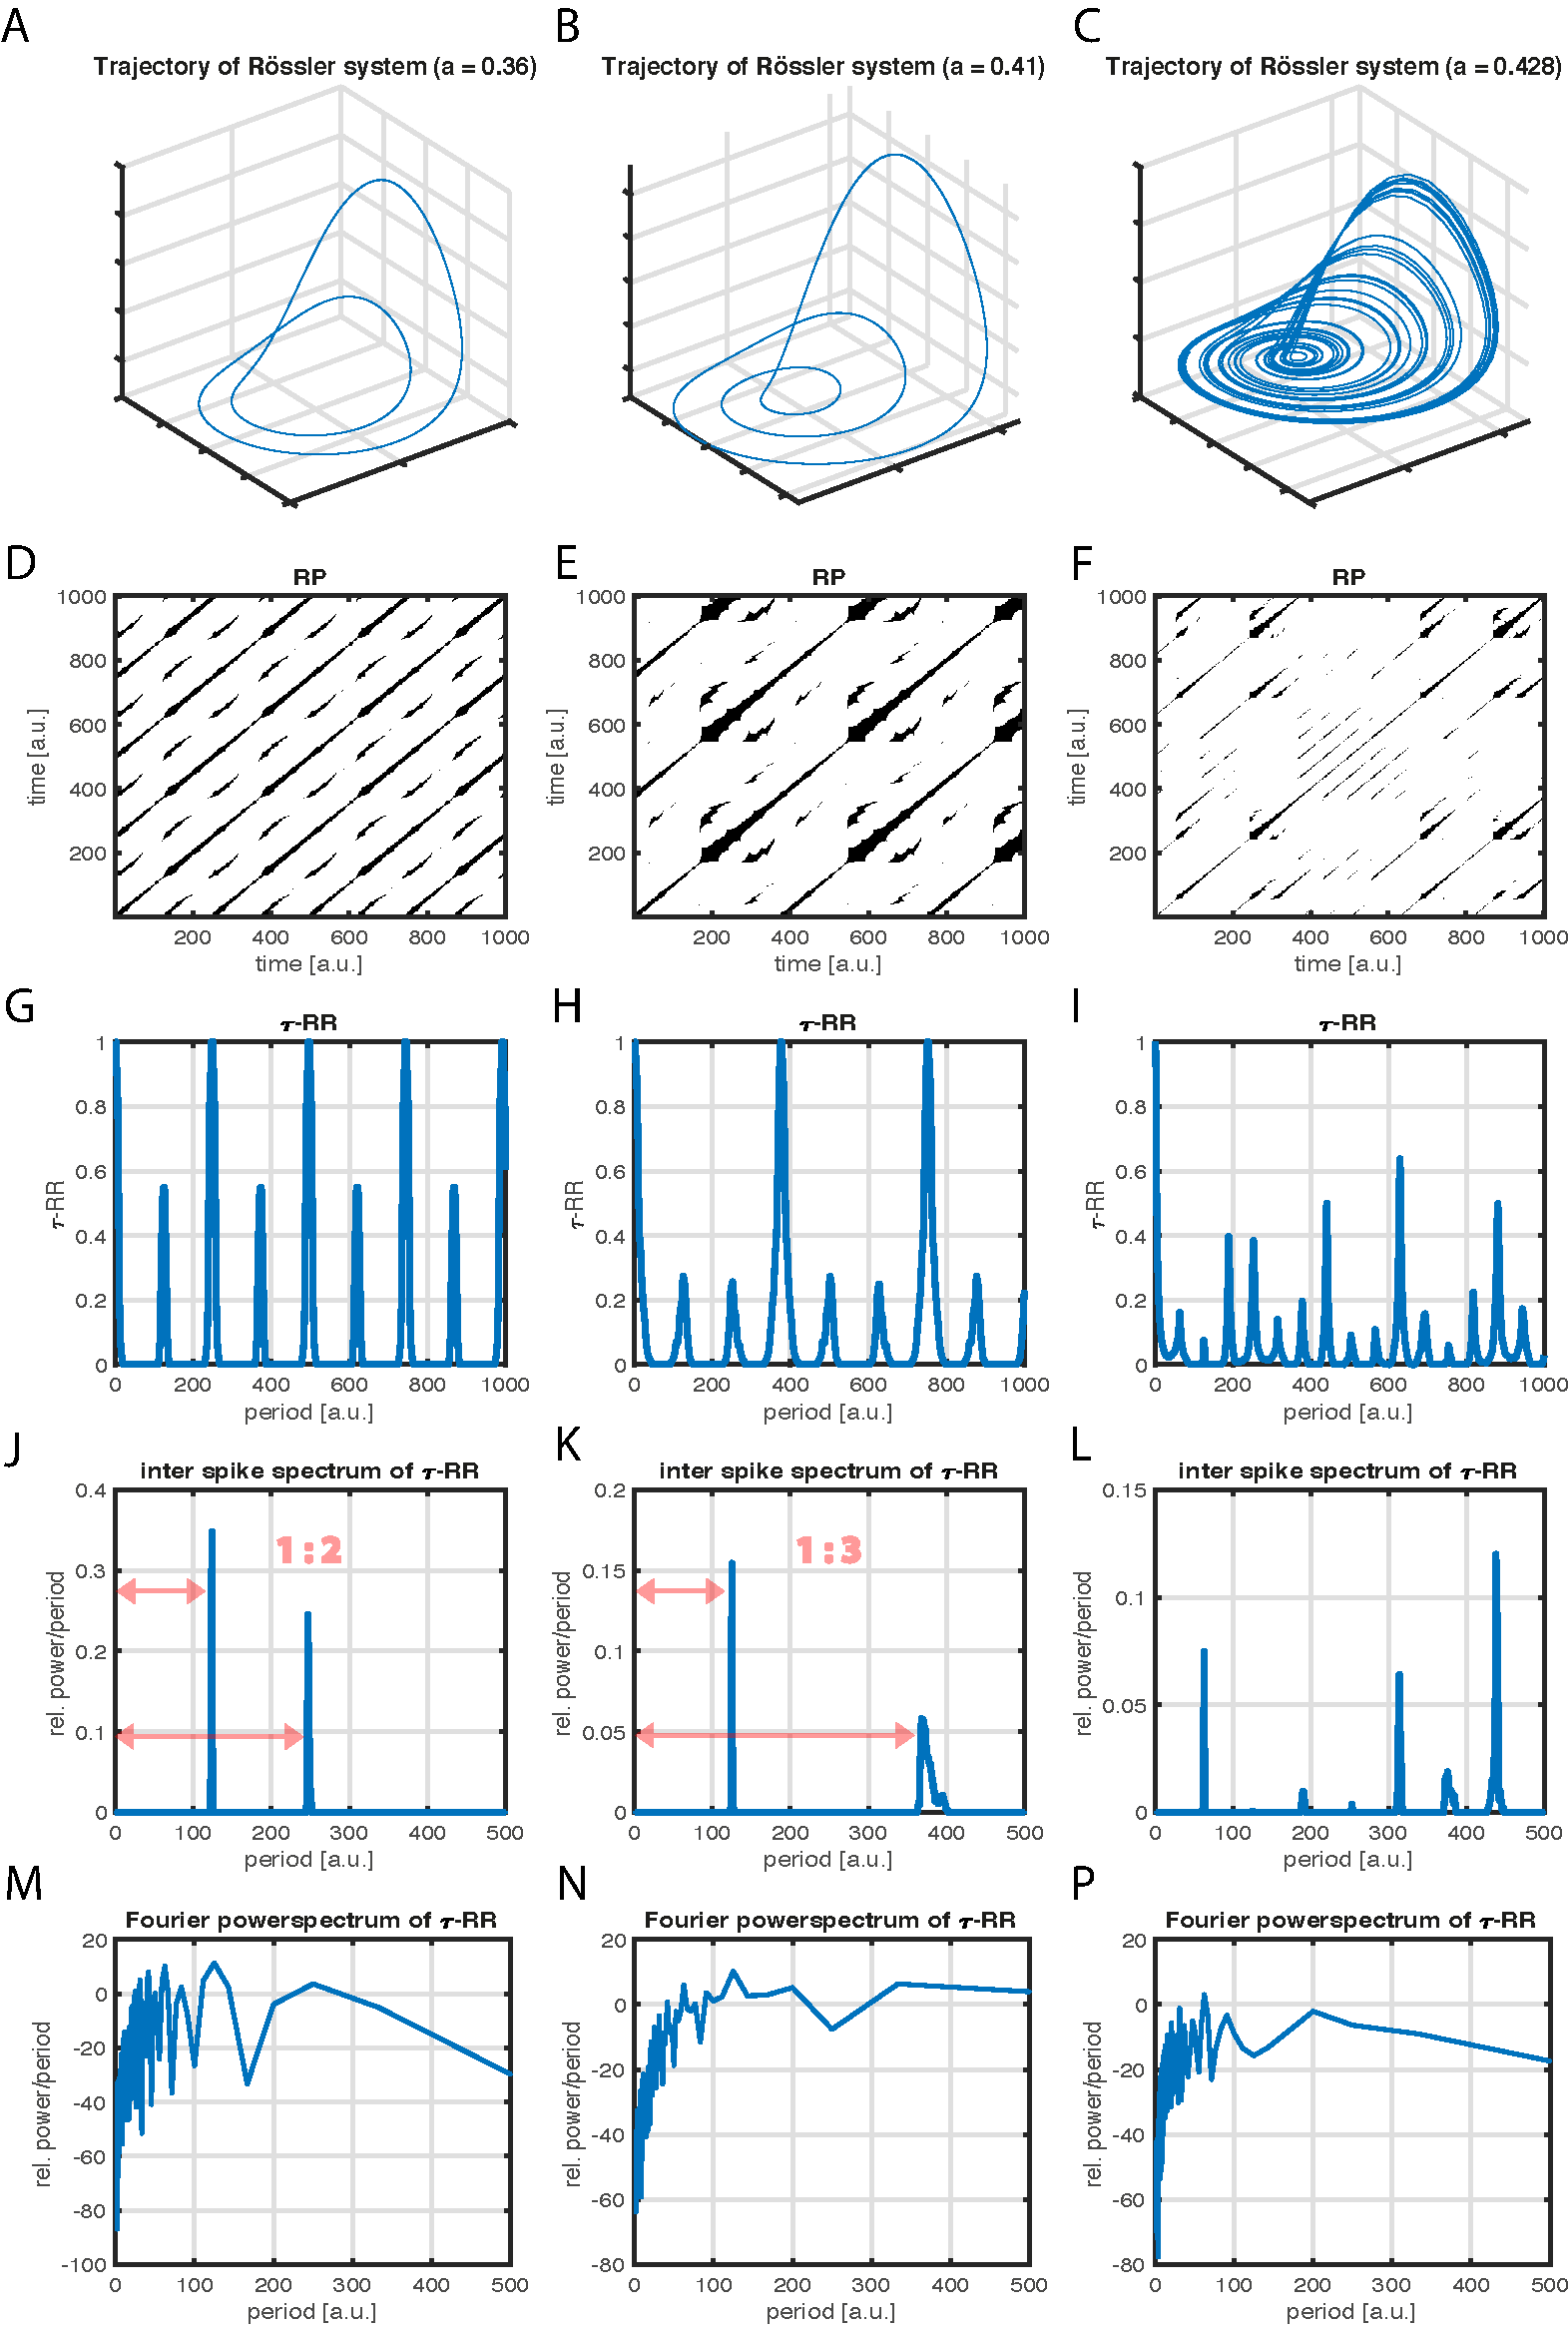
\includegraphics[width=0.9\textwidth]{./figures/fig_tau_rr_example_roessler}
 \caption{Inter spike spectra of the $\tau$-RR of the R\"ossler system in three different dynamical regimes with parameters $b=2$, $c=4$. 
 Trajectory of the system in a \textbf{A} period-2 (parameter $a=0.36$), \textbf{B} in a period-3 (parameter $a=0.41$) and 
 \textbf{C} in a chaotic regime (parameter $a=0.428$). 
 \textbf{D, E, F} The corresponding RPs, obtained by using a recurrence threshold corresponding to a 10\% global 
 recurrence rate for D \& E and 5\% for F. 
  \textbf{G, H, I} $\tau$-RR's of the shown RPs. 
  \textbf{J, K, L} The proposed inter spike spectra of the $\tau$-RR's shown in panels G, H, I. Spectra were obtained with a LASSO regression and a regularization threshold 
  corresponding to $\rho=0.95$ accordance of $\tau$-RR's and re-composed signals. The distance ratio of the peaks reflect the limit cycle dynamic.  
  \textbf{M, N, P} Fourier power spectra of the $\tau$-RR's shown in panels G, H, I.
 }
\label{fig_tau_rr_example_roessler}
\end{figure}

The inter spike spectra unravel the specific dynamics, which are also apparent in the state space portraits (Fig.~\ref{fig_tau_rr_example_roessler}A, B, C) and in the 
$\tau$-RRs (Fig.~\ref{fig_tau_rr_example_roessler}G, H, I). The proposed idea is also 
robust to noise (see Fig.~\ref{fig_tau_rr_example_roessler_noise} in the Appendix). This is because the peaks of the $\tau$-RR are insensitive to noise. While the peak shape does 
change in the presence of noise, its position does not, and this is what the inter spike spectrum encrypts after all.

\subsection{Bifurcations in the Logistic map}

We consider the Logistic map $x_{n+1}=r\cdot x_n \left( 1-x_n \right)$ for changing control parameter $r$. We vary $r$ from $r=3.4$ to $r=4$ in steps of $0.001$. For 
each setting of $r$ 
\begin{itemize}[noitemsep]
\item[(1)] a time series of length $N=201$ is computed with a random initial condition $u_0 \in [0,\ 1]$, neglecting the first $1,000$ samples as transients,
\item[(2)] $100$ iterative Amplitude Adjusted Fourier Transform (iAAFT) surrogates \cite{Schreiber1996,Schreiber2000} are computed,
\item[(3)] the time series and its iAAFT surrogates are embedded in a 2-dimensional state space using a time delay of unity,
\item[(4)] from the 2-dimensional trajectories RPs, Eq.~\eqref{eq_rp_definition}, are computed under a threshold $\varepsilon=0.05$,
\item[(5)] $\tau$-RR, Eq.~\eqref{eq_tau_rr}, is computed from the RP of the signal and from the RPs of the surrogates,
\item[(6)] inter spike spectra are obtained from $\tau$-RR of the signal and from the $\tau$-RRs of the surrogates, see Section \ref{sec_tau_rr_method}, and finally,
\item[(7)] from the distribution of the surrogate inter spike spectra the $95^\text{th}$ percentile is computed. The peaks of the inter spike spectrum of the signal which exceed 
this percentile are counted. 
\end{itemize}
In this example, the according null hypothesis is that the data stems from a process which yields the same auto-correlation, hence the same Fourier powerspectrum, and the same 
amplitude distribution. We consider the number of significant peaks in the inter spike spectrum with
respect to the control parameter in order to distinguish the corresponding dynamics (Fig.~\ref{fig_tau_rr_logistic}C).
A correlation with the positive Lyapunov exponent (Fig.~\ref{fig_tau_rr_logistic}A) is discernible 
($\rho_{\text{Pearson}}=0.72$). Moreover, this analysis can tackle period-doubling, since it ``measures'' the dominant cycles via the inter spike spectrum. 

A less computationally intensive approach is to compute surrogates for the $\tau$-RR analytically, rather than computing a RP and its $\tau$-RR for each iAAFT surrogate of the 
time series. This translates into a null hypothesis 
that the $\tau$-RR and its corresponding inter spike spectrum stems from a RP of a random signal. In this case the probability of finding a black point in the RP can be obtained 
from a binomial distribution with probability parameter $p$ set to the recurrence rate of the RP of the signal. This way $100$ surrogate $\tau$-RRs are computed in step (5). 
The results are even slightly better compared to the ones obtained from the iAAFT surrogates (Fig.~\ref{fig_tau_rr_logistic}B, $\rho_{\text{Pearson}}=0.81$). The first period doubling at 
$r \approx 3.458$ cannot be detected by any of the surrogates.

The described procedure does work well for map data, because most often the $\tau$-RR for those kind of data reveals a ``spiky enough'' nature. 
On the contrary, highly sampled (flow-) data often yield not as 
spiky $\tau$-RR's and, thus, the number of significant peaks in the inter spike spectrum may not be sensitive enough to detect period-doubling bifurcations. Moreover the sensitivity of the 
inter spike spectrum to detect the regime shifts also depends on the critical regularization threshold. Nevertheless the 
according inter spike spectra is still revealing important information (Fig.~\ref{fig_tau_rr_example_roessler}) and practitioners can design appropriate quantifying statistics based 
on these spectra, which suit the 
research task.

\begin{figure}
 \centering
 \includegraphics[width=\textwidth]{./figures/fig_tau_rr_logistic}
 \caption{\textbf{A} Lyapunov exponent of the Logistic map as a function of the control parameter $r$. 
 \textbf{B} Number of significant peaks ($\alpha=0.05$) in the inter spike spectrum of the $\tau$-RR and its Pearson correlation coefficient to the Lyapunov exponent shown in \textbf{A} 
 (white noise surrogates). 
 \textbf{C} Same as \textbf{B}, but for iterative Amplitude Adjusted Fourier Transform (iAAFT) surrogates \cite{Schreiber1996,Schreiber2000}. For obtaining the inter spike spectra we used 
 a LASSO regression and a regularization threshold corresponding to $\rho=0.95$ accordance of $\tau$-RR's and re-composed signals.  
}
\label{fig_tau_rr_logistic}
\end{figure}

\subsection{Inter spike spectra of power grid frequency data}

Power grids are large, synchronized, complex networks whose stable functioning is indispensable for modern societies.
To maintain the stability of a power grid, the balance between energy consumption and energy generation must be ensured. 
In an AC-power grid, the grid frequency is an observable variable that reflects how well this balance is satisfied. 
In this process, the grid frequency and its deviations from the nominal frequency are continuously recorded and monitored by 
the grid operators (in Europe and many parts of the world this is $50$ \si{Hz} or $60$ \si{Hz} in America and, for example, southern Japan).
For example, if there is more (less) demand than supply supply, the network frequency decreases (increases) compared to the nominal frequency \cite{kundur1994power}.
\\
The frequency variations can include other information, such as the functionality of control systems \cite{gorjao2020data}, the effect of fluctuations in
renewable energies (REs), demands on the grid \cite{anvari2020stochastic} and, moreover, the effect of regular dispatches due to the trading market 
\cite{meyer2020identifying}. The latter induce periodic frequency jumps. The frequency trajectory for the Great Britain (GB) and Continental Europe (CE) 
grid shown in Fig.~\ref{} demonstrates clear jumps every hour \todo[inline]{(maybe we should add this figure and one from auto-correlation or $\tau$-RP)}. 
Furthermore, autocorrelation/$\tau$-RP shows the regular peaks every $30$ \si{min} and one hour (see Fig.~\ref{}). These peaks are caused by a mismatch of power 
supply and demand \cite{weissbach2009high} during dispatches. In most electricity grids the
operation of dispatchable power plants is scheduled in one hour blocks, where additional (shorter) $30$ and $15$ \si{min} intervals
might exist. Looking at the frequency spectrum in Fig.~\ref{}, however, does not display sharp peaks exactly at $30$ and $60$ \si{min}. \\

\todo[inline]{Now we should start the story of Inter-spike-spectrum}.


\begin{figure}
 \centering
 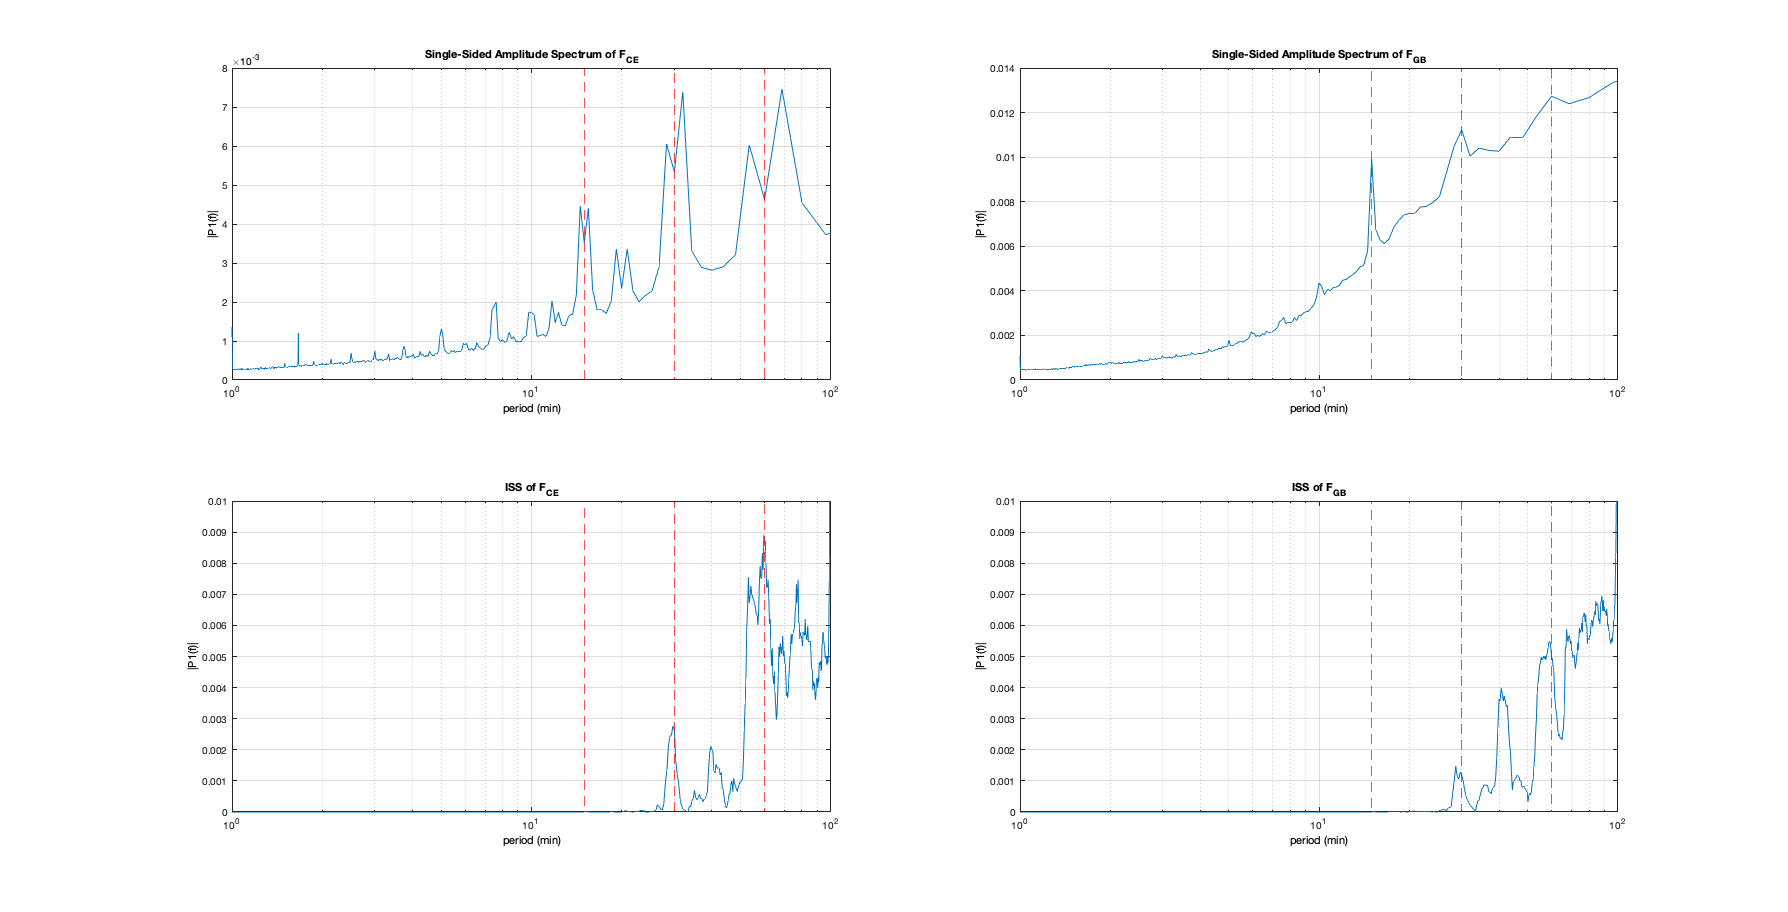
\includegraphics[width=\textwidth]{./figures/fig_power_grid_spectra_lasso_standard_20s}
 \caption{THIS WILL BE A HIGH-RES FIGURE SOON AND A CAPTION WILL BE ADDED  
}
\label{fig_power_spectra_frequency}
\end{figure}

\section{Conclusion}\label{sec_tau_rr_conclusion}

A novel type of powerspectrum, the \textit{inter spike spectrum}, has been proposed. The method decomposes any arbitrary signal into basis functions which consist of (lagged) Dirac 
combs (DC) of different inter-spike period. The loading for each period is obtained by a regularized regression, which promotes sparsity in its solution (we chose LASSO or a sequentially 
thresholded least squares regression STLS). Since there are 
$M = \sum_{i=1}^{\ceil*{N/2}+1}i$ basis functions for a signal of length $N$ the regression can get computationally intensive for $N>1,000$. When plotting the computed loadings as a function 
of the period (or frequency) the inter spike spectrum is obtained. This novel powerspectrum is superior to an ordinary FFT-based powerspectrum, when the signal has a spike-train-like 
appearance. Due to the sparse regression underlying the method, there is no unique inverse of the transformation and the regularization parameter plays a crucial role and determines the 
appearance of the obtained inter spike spectrum. Moreover, similar to the Nyquist frequency barrier in the Fourier Transform which sets a lower bound for the corresponding wave period, here 
the maximum considered inter spike period is bounded by $T_{\text{is}}^{\text{max}} = \ceil*{N/2}+1$.

The invention of the proposed method has been motivated by the idea of transforming $\tau$-recurrence rate signals ($\tau$-RR's) into their frequency domain. 
This general idea \cite{Zbilut2008} allows for a frequency analysis of high dimensional systems, because the RP is a representation of the system's state space trajectory.   
The $\tau$-RR of a recurrence plot (RP) usually has a spiky shape, especially for map-like data, and the inter spike spectrum can reliably reveal the system's dominant frequencies, 
which is not possible when Fourier transforming the $\tau$-RR or the underlying signal itself. Since the position of the peaks 
in the $\tau$-RR are not sensitive to noise, the corresponding inter spike spectrum also yields robust results in the presence of noise. We have successfully used the idea 
of transforming the $\tau$-RR for the detection of bifurcations in the Logistic map. By constructing appropriate surrogates of the inter spike spectra, and thus a null model, 
the number of significant peaks in the inter spike spectrum correlated well with the positive Lyapunov exponent. This measure was also able to resolve period-doubling bifurcations. 
\todo[inline]{Here a quick summary of the other applications.}

We could think of a broad range of applications of the proposed idea. The inter spike spectrum itself can serve as a valuable tool for the analysis of any sort of 
spike-train-like data. On the other hand, the inter spike spectrum of the $\tau$-RR of a signal can serve as a generalized, nonlinear frequency analysis tool for complex systems. 
When there is only a subset of state variables available, the state space has to be reconstructed as a pre-processing step. Recent findings \cite{Kraemer2021,Kraemer2022} show that 
this reconstruction process can be reliably automated and applied to multivariate data as well. This would allow for a ``running window'' approach, in order to detect transitions. 
Due to the mentioned computational constraints of our proposed method, a window size $w\leq 1,000$ would possibly suffice for most data, especially when it is map-like, i.e., not 
highly sampled.  


\begin{acknowledgements}
This work has been financially supported by the German Research Foundation (DFG projects MA4759/8 and MA4759/9). All computations have been carried out in MATLAB\textsuperscript{\textregistered} 
and the Julia language and made use of the packages \textit{DynamicalSystems.jl} \cite{datseris2018} and \textit{DifferentialEquations.jl} \cite{rackauckas2017}.
\end{acknowledgements}


% Authors must disclose all relationships or interests that 
% could have direct or potential influence or impart bias on 
% the work: 
%
\section*{Conflict of interest}

The authors declare that they have no conflict of interest.
 
\section*{Code availability}

The study that we present here is available as a fully reproducible code base
**Repository will be published and cited here, when accepted** and the method
will be available in the Julia language **Package will be published and cited here, 
when accepted** and as a MATLAB\textsuperscript{\textregistered} toolbox 
**Toolbox will be published and cited here, when accepted**.

\clearpage
\appendix
\section{Inter spike spectra for noisy R\"ossler system}

\begin{figure}[h!]
 \centering
 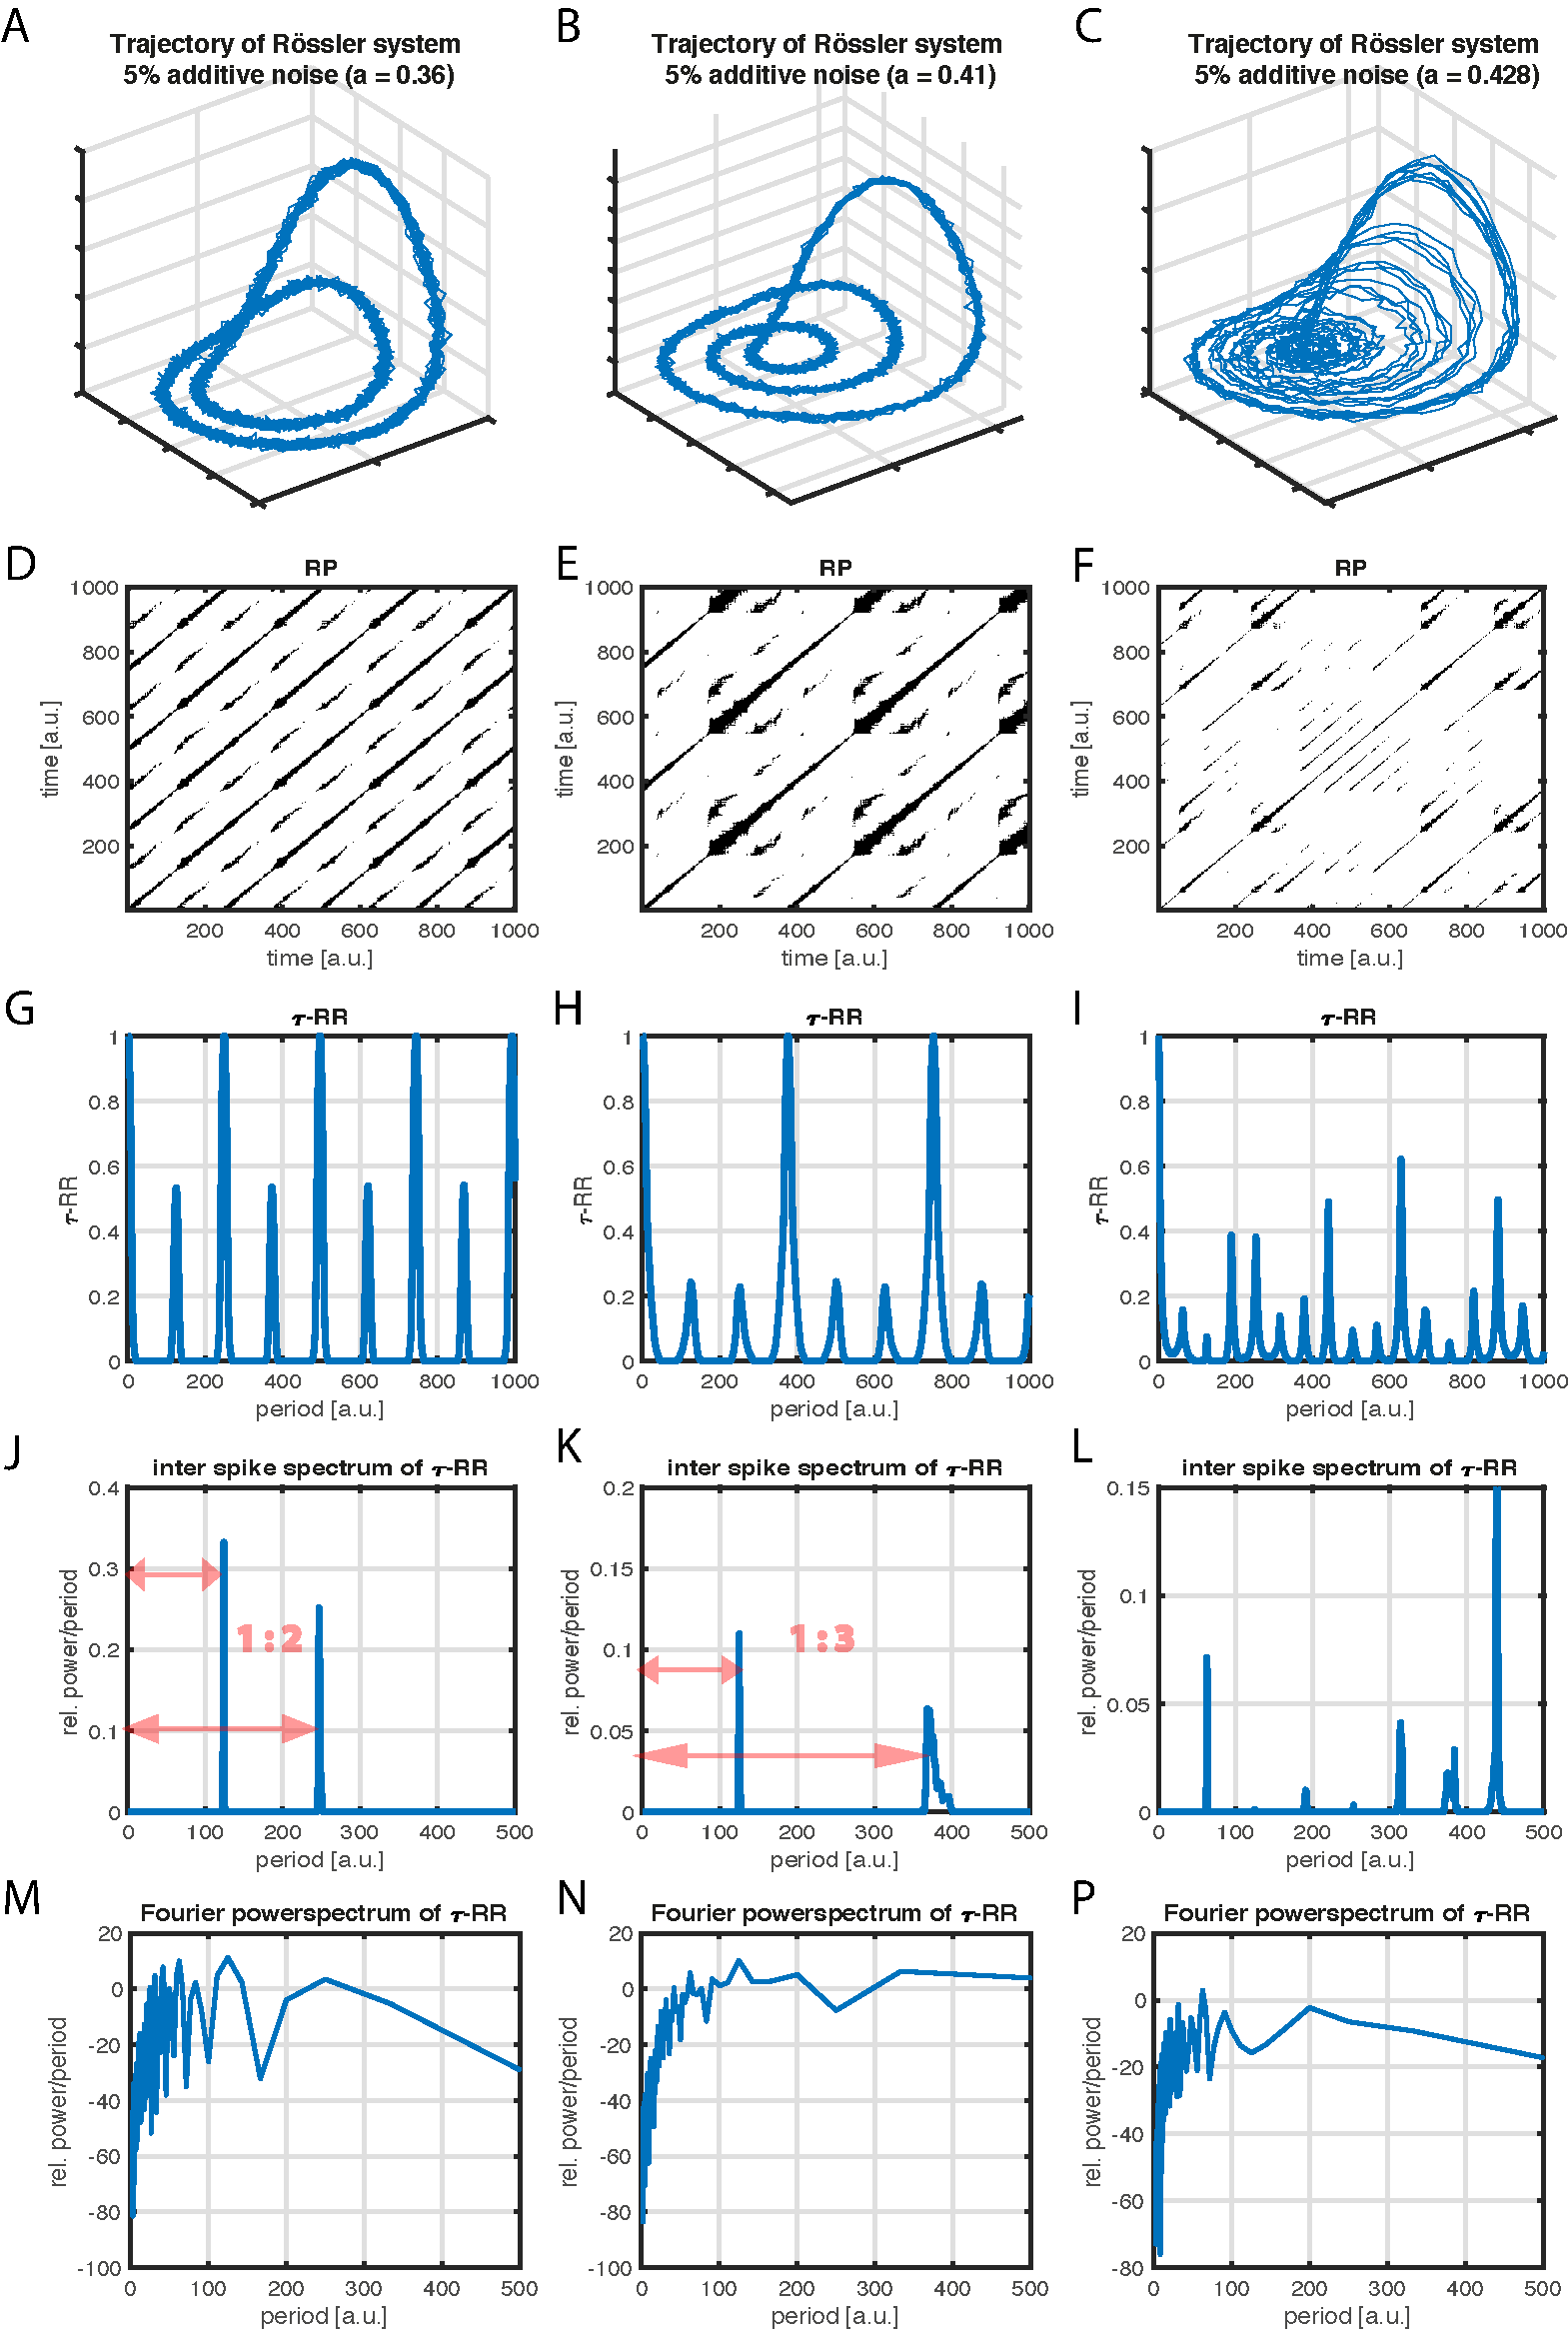
\includegraphics[width=0.9\textwidth]{./figures/fig_tau_rr_example_roessler_noise}
 \caption{Same as in Fig.~\ref{fig_tau_rr_example_roessler}, but here with 5\% additive Gaussian white noise. The appearance of the inter spike spectra 
 in \textbf{J, K, L} and the Fourier spectra in \textbf{M, N, P} are unaffected by the additive noise noise.
 }
\label{fig_tau_rr_example_roessler_noise}
\end{figure}

\section{Exemplary models}
 
\subsection{Lorenz system}\label{sec_models_lorenz63}

The classical Lorenz-63 system \cite{lorenz1963} is defined as

\begin{equation}
\begin{array}{rcl}
\dot{x}&=&\sigma(y-x) \\
\dot{y}&=&x(r-z)-y \\
\dot{z}&=&xy - \beta z.
\end{array}
\label{eq_model_Lorenz63}
\end{equation}

\noindent For producing Fig.~\ref{fig_tau_rr_spectrum_example} we set the initial condition to $u_0=[0.0, 10.0, 0.0]$, used a sampling time of $\Delta t=0.01$ and discarded the first 
2,000 points of the integration as transients. The parameters have been set to 
$\sigma=10, \beta=8/3, \rho=28$ and we used a time series consisting of 6,000 samples.

\subsection{R\"ossler system}\label{sec_models_roessler}

The R\"ossler system \cite{roessler1976} is defined as
\begin{align}
\begin{array}{rcl}
\dot{x}&=&-y-z \\
\dot{y}&=&x+ay \\
\dot{z}&=&b+ z(x-c) .
\end{array}
\label{eq_model_roessler}
\end{align}
For producing Figs.~\ref{fig_tau_rr_example_roessler_noise},~\ref{fig_tau_rr_example_roessler} the initial condition for producing panels \textbf{A} \& \textbf{B} was set to $u_0=[.7, -1, 0.4]$ with a sampling time 
of $dt=0.05$ and in case of panel \textbf{C} $u_0=[-0.1242, -2.5415, 0.2772]$ with a sampling time of $dt=0.1$. The first $5,000$ samples were discarded as transients and trajectories of length $N=5,000$ were 
obtained from which we computed the RPs and the corresponding $\tau$-RR's. For the inter spike spectra only the first $1,000$ values of the $\tau$-RR's were considered.
 


% BibTeX users please use one of
%\bibliographystyle{spbasic}      % basic style, author-year citations
%\bibliographystyle{spmpsci}      % mathematics and physical sciences
%\bibliographystyle{spphys}       % APS-like style for physics
%\bibliography{}   % name your BibTeX data base

% Non-BibTeX users please use
\bibliographystyle{spbasic} 
\bibliography{inter_spike_bib}


\end{document}
% end of file 

